\section{Introduction and Literature Review}
%TODO:
%Re-phrase introduction

%Add analysis to MDA, D miner, Tokyo ping, zeph

%Add discussion to possible work section


%Introduction which sets the scene
%for the research proposal and puts the research in context.
\subsection{Introduction}
The importance and impact of the internet over the past 30 years cannot be overstated; in almost every area it has dramatically changed the efficiency with which data can be transmitted and received across the globe. In order to facilitate such a large system, many millions of nodes are interlinked, all working together in tandem to send and receive "packets" of data. 

Network topology is defined as the physical and logical layout of nodes and connections in a network, with nodes usually being either a router, switch or software emulating a switch or router. 

Being able to map the topology of this structure is key not only to establish the most efficient routes for data transmission by reducing latency but also to ensure even traffic distribution across different network paths via Load balancing. There are also additional advantages of accurate mapping, which include mitigating potential security threats, fault detection and scalability. A common tool used to achieve this is Traceroute, with it being widely used, from the diagnosis of network
problems to the assemblage of internet maps. \cite{anomalies}


\subsection{Literature Review}
%Description and critical discussion of
%research context relevant to the chosen
%research context.

%-------------------------------------------------------
%Traceroute
Traceroute reports an IP address for each network-layer device along the path from a source to a destination host in an IP network\cite{jacobson1989traceroute}. However, traceroute fails in the presence of routes that employ load balancing on packet header fields. The failures lead to incorrect route inferences that may mislead operators during problem diagnosis and result in erroneous internet maps.\cite{anomalies}\cite{exhaustive}

%Analysis
Jacobson's traceroute, released in 1989 was the \textit{de facto} tool used for network diagnostics and internet topology mapping, however as stated above it cannot properly map routes which use load balancing for packet header fields. This severely impairs it's ability and overall feasibility as load balancing is widely used.

%-------------------------------------------------
%Load balancing
Load balancing is used to increase dependability and enhance resource usage. With intra-domain routing protocols OSPF\cite{moyospf} and IS-IS\cite{isis} being used to implement this. Routers can spread their traffic across multiple equal-cost paths using a per-packet, per-flow or per-destination policy. \cite{cisco}\cite{juniper} For per-flow balancing packet header information ascribes each packet to a flow, and the router forwards all packets belonging to a same flow to the same interface. A natural flow identifier is the classic five-tuple of fields from
the IP header and either the TCP or UDP headers: Source
Address, Destination Address, Protocol, Source Port, and
Destination Port. Per-flow load balancing ensures that packets from the same flow are delivered in order. Per-packet load balanc- ing makes no attempt to keep packets from the same flow together, and focuses purely on maintaining an even load.
Per-destination load balancing could be seen as a coarse form of per-flow load balancing, as it directs packets based upon the destination IP address. But, as it disregards source in-153
formation, there is no notion of a flow per se.\cite{anomalies}

%Analysis
When load balancing in employed there is no single route from a source to a destination, for example with per-load packet balancing any given packet could go any one of a selection of possible routes. Although, with per-flow load balancing a single route is still used for packets of a given flow, however even in this case differing flows for the same source and destination pair can follow different possible routes. 
%----------------------------------------------------
%Problems with traceroute
As stated above, the original traceroute is insufficient to correctly recognize individual routes from a group of routes. This is due to how traceroute traverses routes in a network; it discovers hops along a route with a series of probe packets with increasing TTL, with each node in the network sending back an ICMP packet back in response. If these probe packets reach a router using load-balancing there is a possibility of the probe packets being directed along different paths, potentially resulting in missing nodes/links and false links as shown below in fig. \ref{figure:missing_node_fig}.

\begin{figure}[h!!]
  \begin{center}
    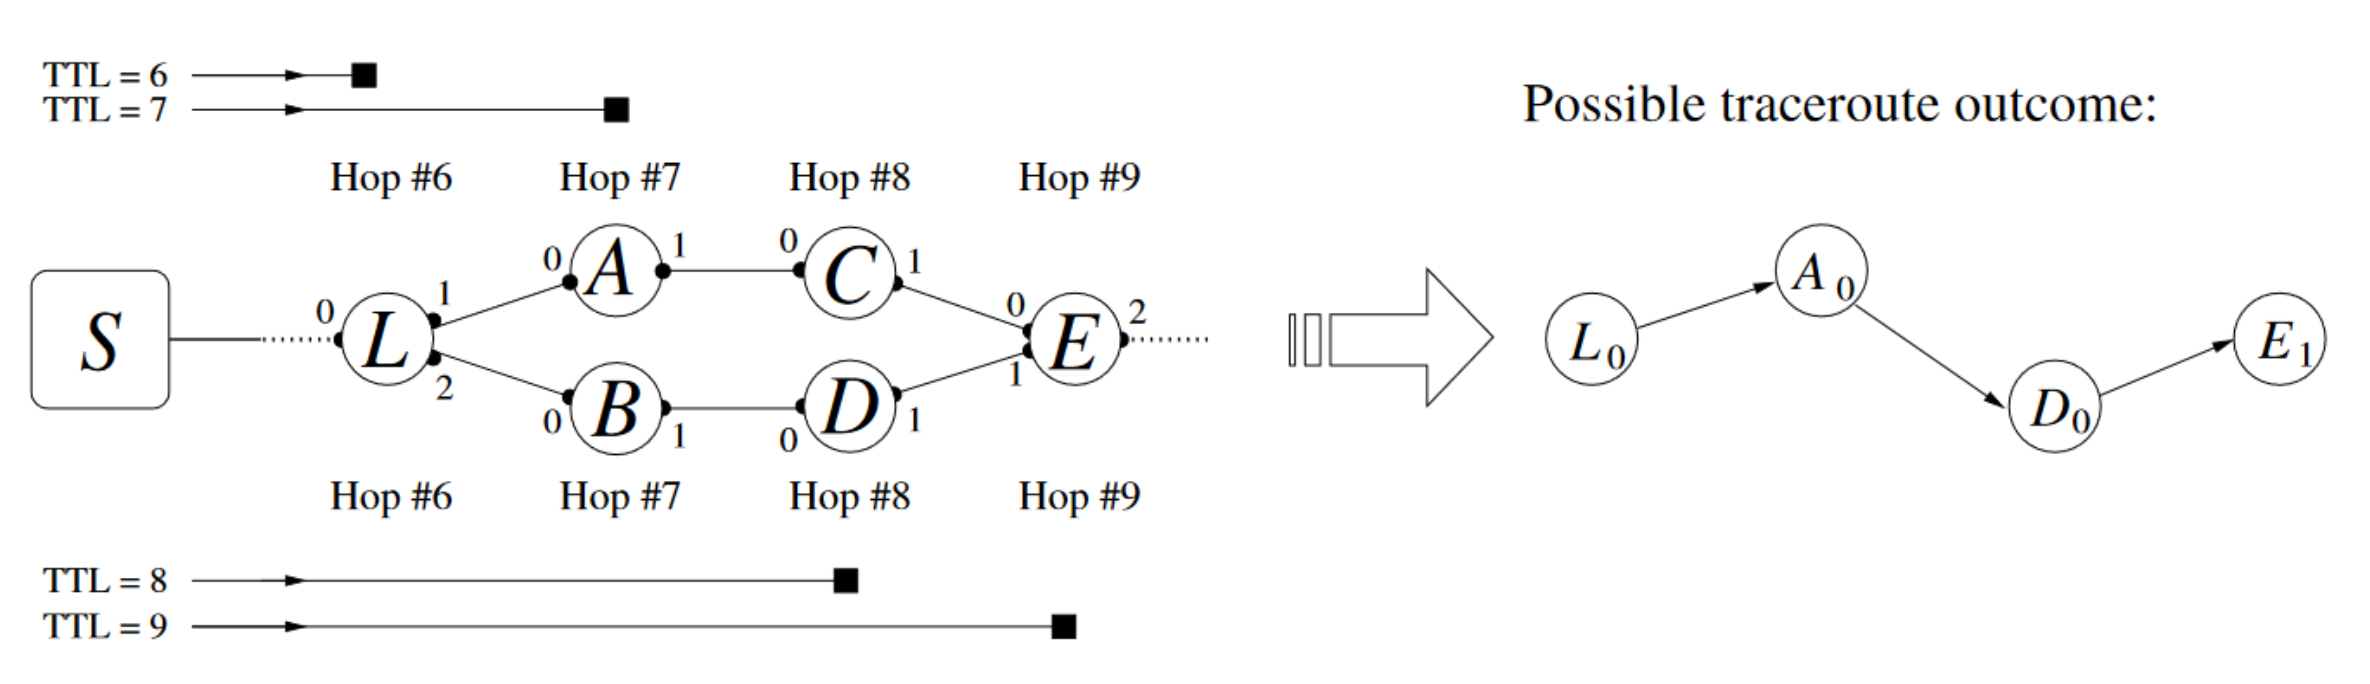
\includegraphics[scale=0.3]{images/missing_nodes.png}
    \caption{Missing nodes and links, and false links \cite{anomalies}}
    \label{figure:missing_node_fig}
  \end{center}
\end{figure}


%----------------------------------------------------
%Different network topology types and their implications

Due to the large prevalence of routers using Load balancing this is highly problematic, in response to this, new approaches have been proposed to mitigate the issue's highlighted above.
%-------------------------------------------------------
%Paris trace route
Paris traceroute, a new traceroute designed
for networks with load balancing routers. Its key innovation is to control the probe packet header fields in a manner that allows all probes towards a destination to follow the same path in the presence of per-flow load balancing. It also allows a user to distinguish between the presence of per-flow load balancing and per-packet load balancing. Unfortunately, due to the random nature of per-packet load balancing, Paris traceroute cannot perfectly enumerate all paths in all situations. But it can do considerably better than the classic traceroute, and it can flag those instances
where there are doubts. \cite{anomalies}

\begin{figure}[h!!]
  \begin{center}
    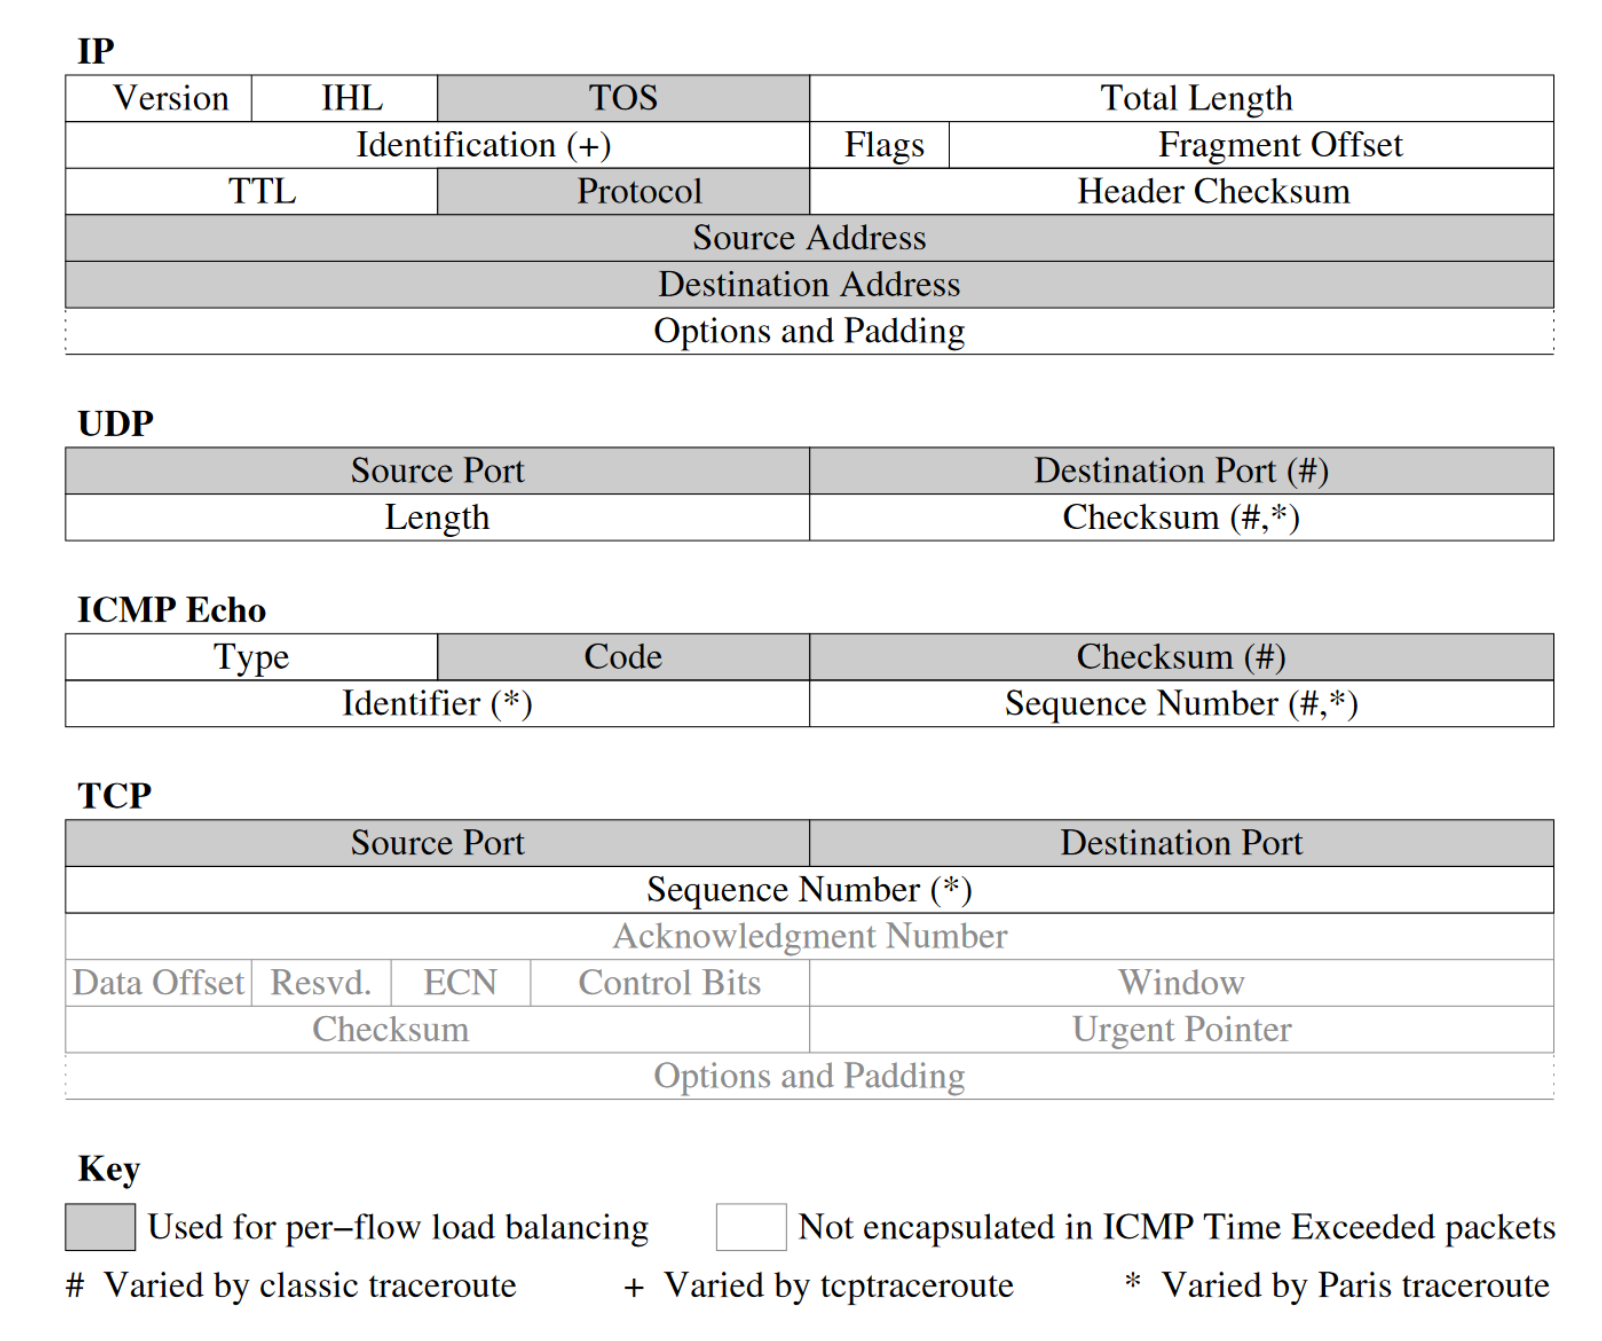
\includegraphics[scale=0.3]{images/packet_header.png}
    \caption{The roles played by packet header fields \cite{anomalies}}
    \label{figure:packet_header_fig}
  \end{center}
\end{figure}

Paris traceroute controls the flow of each packet allowing them to follow the same path by varying the first eight octets of the transport-layer header, but that are not used for load balancing. For UDP probes, Paris traceroute varies the Checksum field. This requires manipulating the payload to yield the desired value, as packets with an incorrect checksum are liable to be discarded. For ICMP Echo probes, Paris traceroute varies the Sequence Number field, as does classic traceroute, but also varies the Identifier field, so as to keep constant the value for the Checksum
field. Paris traceroute also sends TCP probes, unlike classic traceroute, but like Toren’s variant tcptraceroute. \cite{anomalies}\cite{tcptraceroute}
%Analysis
Paris traceroute is a much more robust tool to map internet topology than traceroute as it can mitigate the effects of per-flow load balancing and ensure packets flow on the correct path through the network nodes, avoiding potential missing nodes/links and false links. However, nodes which use Network Address Translation(NAT) can still be problematic for paris traceroute due to the NAT modifying the source/destination IP addresses in the packet headers, obscuring the packet information and also therefore the actual routing path.

%-------------------------------------------------------
%MDA
The Multipath Detection Algorithm (MDA) provides an extension to Paris traceroute called the MDA, a stochastic probing algorithm that adapts the number of
probes to send on a hop-by-hop basis in order to enumerate all reachable interfaces at each hop. The number of probes required by the MDA is a function of a tunable parameter, which is an upper bound on the probability of failing to discover the entire explorable multipath route, or multipath. Upon completion, the MDA yields a level of confidence in its result. The MDA also has mechanisms to deal with unresponsive routers and for identifying per-packet load balancers and routing changes.\cite{MDA2} The MDA works on the basis of an open set of vertices, each of which has been discovered but has not yet had its successor vertices identified. A discovery round consists in choosing a vertex v from the open set and trying to find all of its successors. Where there is no load balancing, v has just one successor, but if v is the responding interface of a load balancing router, there will be two or more possible successors that can only be identified by stochastic probing. In the case that concerns us, per-flow load balancing, successors are found by varying the flow identifier from one probe packet to the next. \cite{MDA-lite}\cite{diamond-miner}\cite{MDA3}
%Analysis
Rather than send a set amount of probes per hop like the original traceroute which sends 3, the MDA varies this amount based on a controllable parameter. The parameter is the upper limit of the probability of not revealing the entire multi-path network. This is highly advantageous as it can adapt to any given network structure, which in the "real" internet can be extremely complex and have many paths, but also due to it's adaptability it can still remain relatively lightweight. However, as it is a stochastic algorithm there is an element of uncertainty to the produced result, this is accounted for by "yeilding" the  confidence of the final output to provide some further information about the validity of the result.

The MDA-Lite, however, reserves node control for particular cases and proceeds hop by hop in the general case. At each hop it seeks to discover all of the vertices at that hop, and in doing so discovers some portion of the edges between that hop and the prior hop. It then seeks out the remaining edges. It operates on the assumption that the diamonds that it encounters will be uniform and unmeshed. If this assumption holds, hop-by-hop probing will maintain the MDA’s failure probability bounds. Because these two topology assumptions might not hold, the MDA-Lite tests for a lack of uniformity and the presence of meshing using methods that are less costly than full application of the MDA. When it detects a diamond that does not adhere to one of the assumptions, it switches to the MDA.\cite{MDA-lite}
%Analysis
MDA-lite is a further improvement on the MDA algorithm by reducing overhead, whilst still having the same performance. It achieves this by operating based on the assumption of uniform hops, with probes being sent at each hop without node control. One flow identifier from each previously discovered vertex in the preceding hop are reused, continuing with additional previously-used flow identifiers and
then new ones. It applies the MDA’s stopping rule to remain within
the MDA’s failure probability bounds for vertex detection. \cite{MDA-lite}

\begin{figure}[h!!]
  \begin{center}
    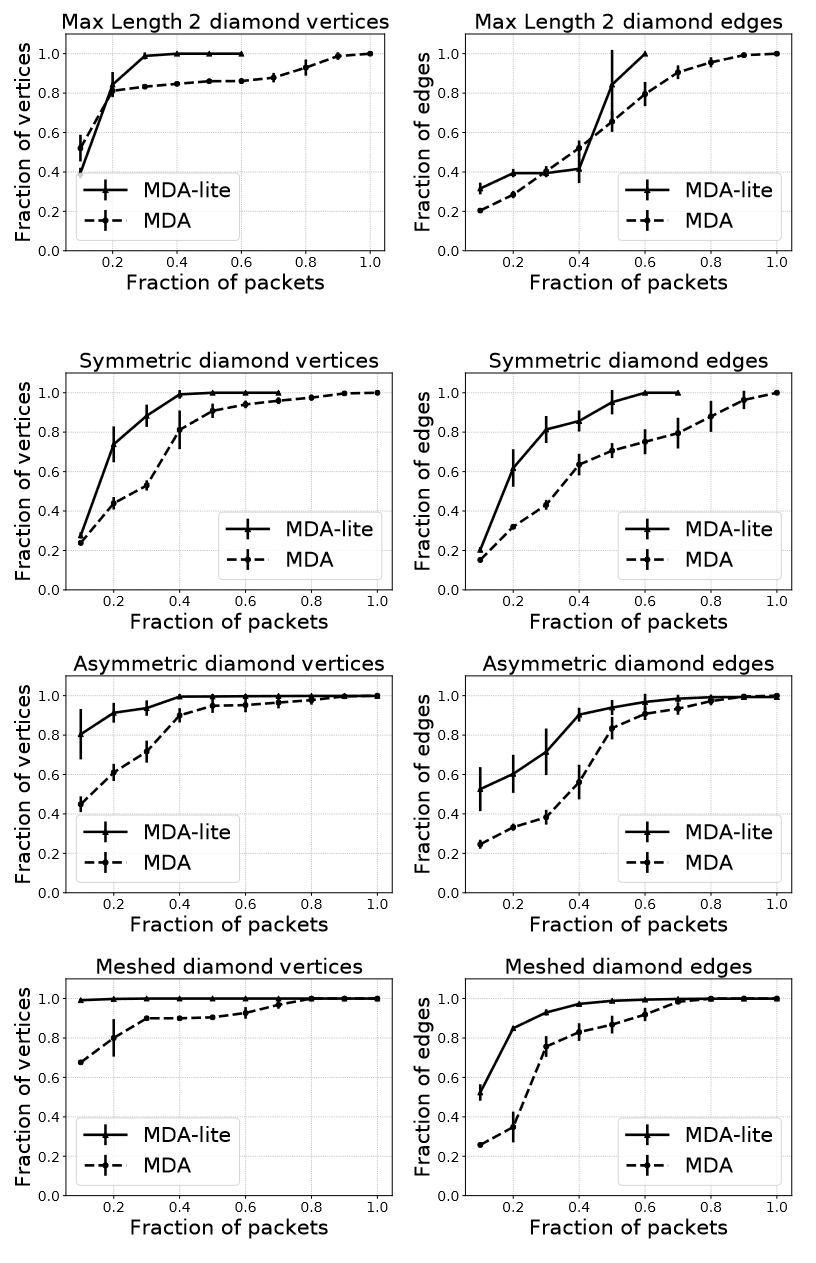
\includegraphics[scale=0.3]{images/MDA_lite.png}
    \caption{MDA-Lite versus MDA simulations\cite{MDA-lite}}
    \label{figure:MDA_lite_fig}
  \end{center}
\end{figure}

%-------------------------------------------------------
%Diamond miner
D-Miner is designed to capture Internet topology snapshots
inclusive of all load-balanced paths. At its heart, D-Miner
uses Yarrp’s randomized and stateless probing to achieve high
probing rates. To this, it adds probe set generation logic that
keeps track, on a per-node basis, of whether all outbound load-
balanced edges have been discovered with high probability.
The logic guides Yarrp through multiple rounds until the full
discovery criterion has been satisfied for almost all nodes. \cite{diamond-miner}

\begin{figure}[h!!]
  \begin{center}
    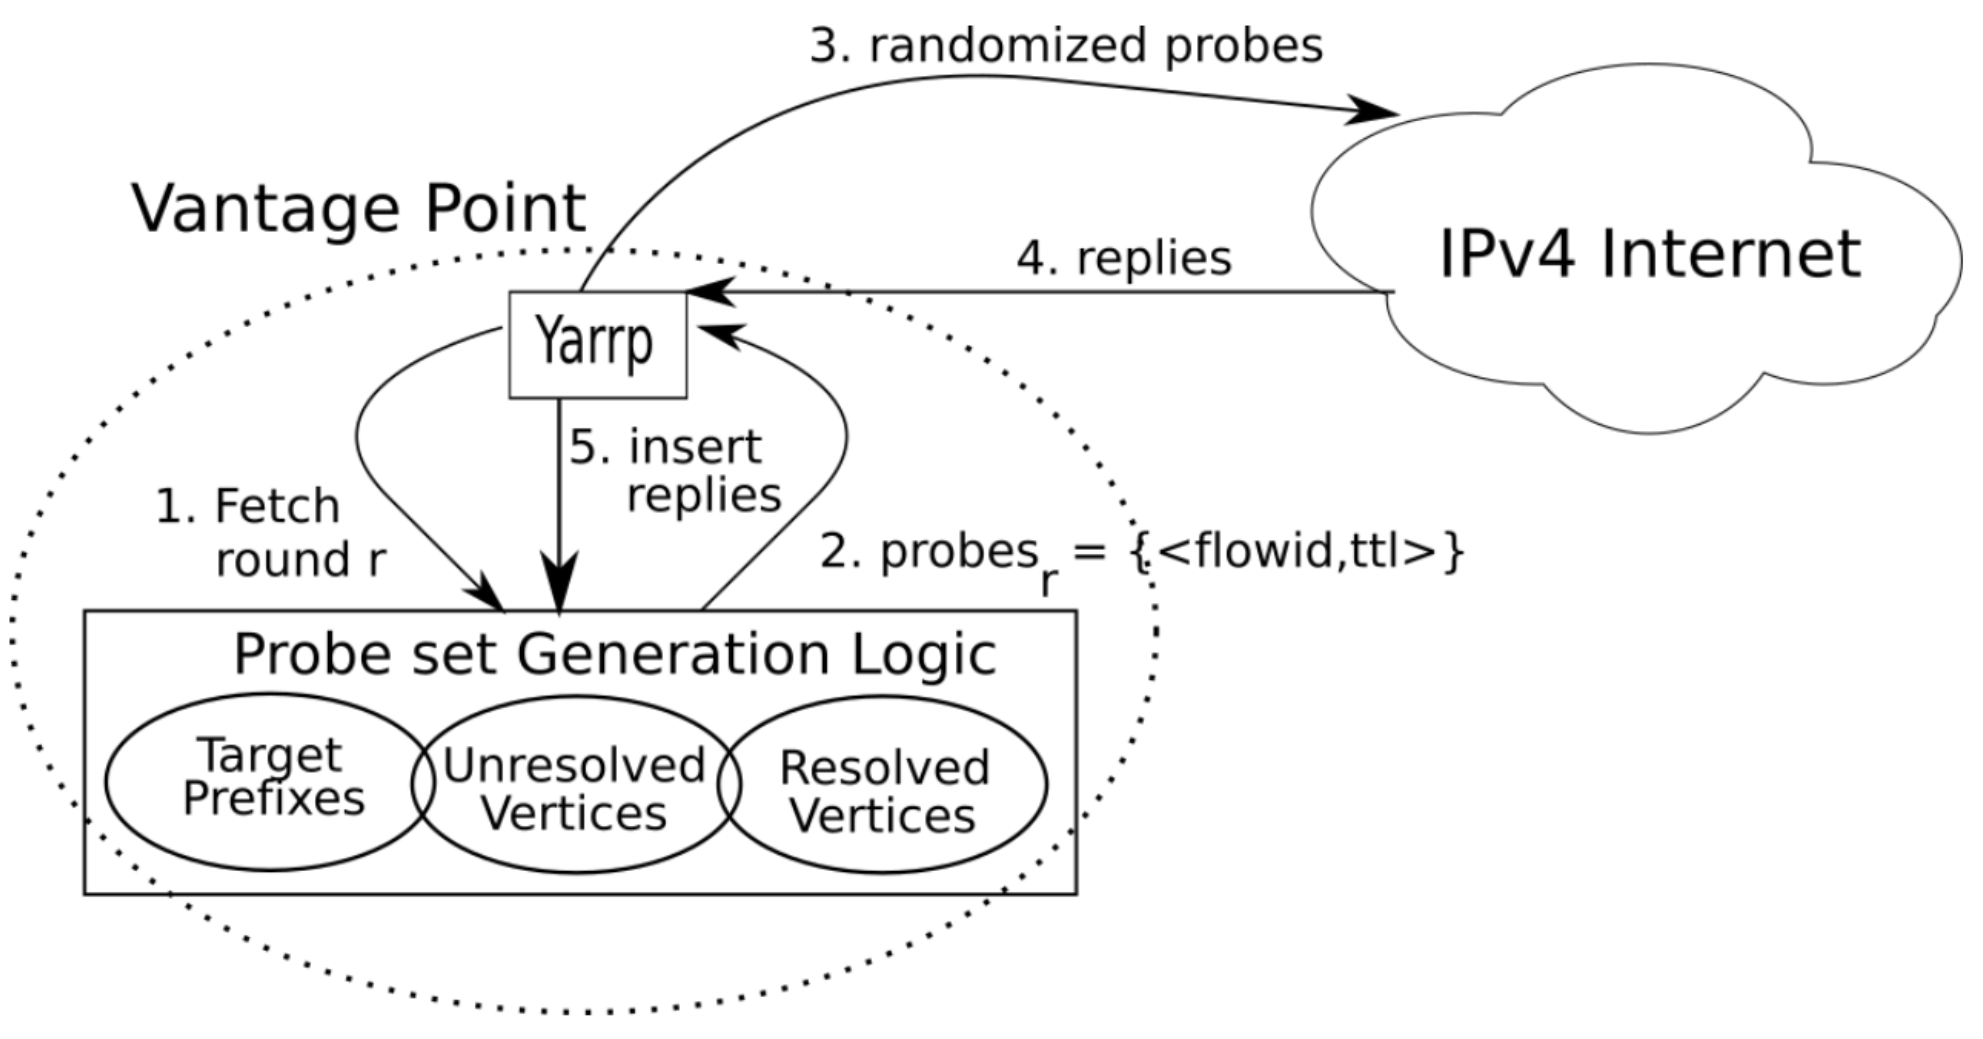
\includegraphics[scale=0.3]{images/diamond.png}
    \caption{Diamond miner high-level conceptual overview \cite{diamond-miner}}
    \label{figure:dminer_overview_fig}
  \end{center}
\end{figure}

%Analysis
Due to Diamond miner's utilisation of Yarrp's randomized and stateless probing, wide coverage of internet topology is achieved. It's incorporation of probe set generation logic allows tracking of  all outbound load-balanced edges from each node with high certainty. D-
Miner permits discovery of the Internet’s multipath topology
in 2.5 days when probing at 100kpps. This high speed allows
us to characterize and quantify dynamic behaviors of the In-
ternet induced by load balancing. Finally, D-Miner enables
for the first time an Internet Scale survey of load balancing
that shows its widespread prevalence, both in the core and at
the edge. \cite{diamond-miner}

%------------------------------------------------------
%Yarrp
The high-level idea of Yarrp is: i) randomization of the probing order of the domain of network range(s) and TTLs; and ii) stateless operation, whereby all necessary state is encoded into the probes such that it can be recovered from the ICMP replies.\cite{yarrp}

\begin{figure}[h!!]
  \begin{center}
    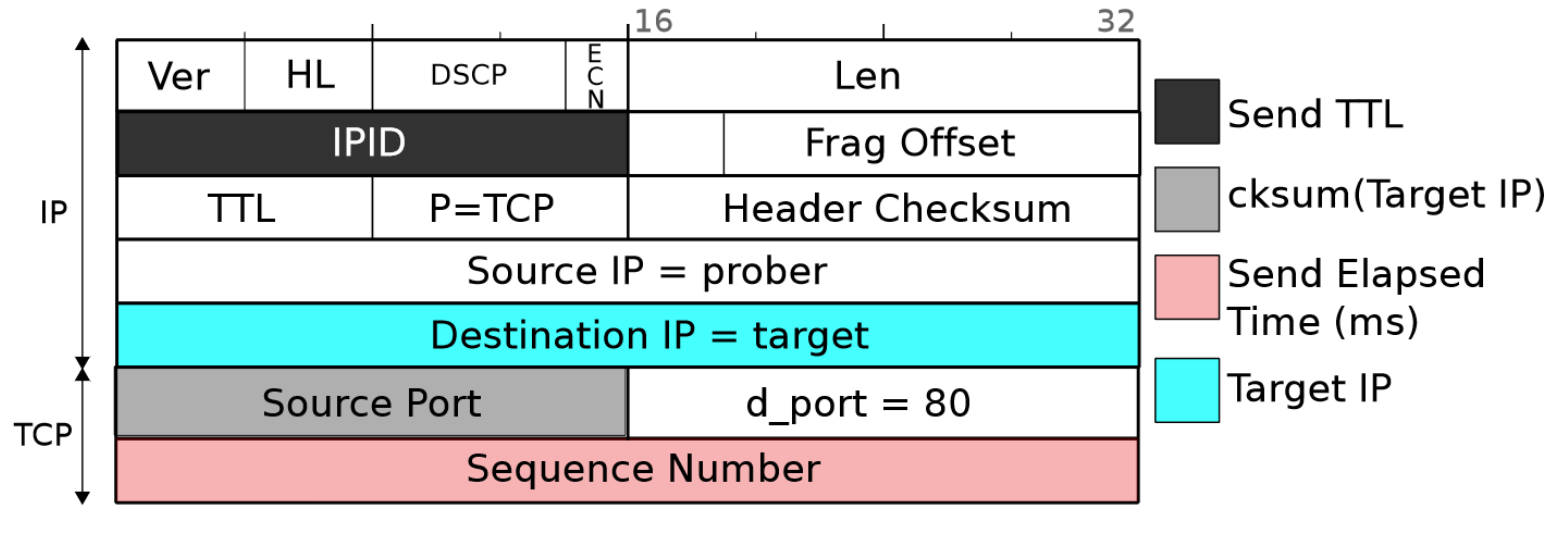
\includegraphics[scale=0.3]{images/yarrp.png}
    \caption{Yarrp encodes information in the IP and TCP field of outgoing proe packets in order to permit stateless operation \cite{yarrp}}
    \label{figure:yarrp_fig}
  \end{center}
\end{figure}

%Analysis
Yarrp enables high speed collection of network topology data, due to it's stateless operation and randomization of the probing order of the domain of network ranges and TTL of ICMP packets sent.

%-------------------------------------------------------
%Dublin traceroute
To detect NATs, Dublin Traceroute forges a custom IP ID in the outgoing packets, and keeps track of them in the response packets. If the response packet references an outgoing packet with different source/destination IP addresses and ports, this may indicate the presence of a NAT. In that case, the packet referenced in the response will be different from the one that was sent, and cannot be correlated anymore. However, the IP ID is expected to be unchanged (thanks to the presence of the don't-fragment bit), and it will contain a value to correlate it to one of the outgoing packets.\cite{dublin_website} \cite{dublin}
Dublin traceroute solves the NAT problem which was a limitation of paris-traceroute, it is also implmeneted in C++ for it's core and has also improved on further limitations of paris traceroute such as memory safety increasing it's robustness. Furthermore, it also offers a python library and interface as a wrapper on top of the C++ codebase. Results are exported as JSON data allowing ease of integration within other applications, adding to it's modularity and usability.


%--------------------------------------------------------
%Zeph map alogrithms
Zeph proceeds across a series of cycles, with
the directives for each cycle being based in large part upon the
success of the directives that were used in the previous cycle. New
directives are also tried out each cycle, with the overall aim being
to improve the completeness of coverage over successive cycles. In
reinforcement learning terms, the reuse of directives is exploitation
and the trying out of new directives is exploration.
Zeph’s challenge is to best use the probing budgets of its agents,
i.e., choose which directives to issue to each agent so as to obtain
the overall most complete route trace picture possible within a
cycle. There are many ways of conceiving of “completeness”, and
the one adopted here is to maximize coverage of the traceroute-
style directed links that are available to be discovered, a directed
link consisting in an ordered pair of IP addresses.\cite{zephMap}

%Analysis 
By applying reinforcement learning for distributed tracing of network routes, zeph discovers the probing directives to allocate to the vantages points in order to maximize topology discovery. 



%----------------------------------
%Clear links from the conclusions of
%literature review to the research questions
%presented in Section 2

\subsection{Possible work}
%Possible improvements which could be carried out for the project
Based on the studied literature above there are several avenues of research which could be carried out to provide potentially fruitful results. Such as expanding upon the existing dublin traceroute implementation to include features such as the Multipath Detection Algorithm and zeph algorithm, and also support for TCP, ICMP and DNS probes in order to create the optimal traceroute tool which improves upon the previous tools such as traceroute and paris traceroute. With these improvements implemented, there could be scope to conduct an internet-wise topology survey as additional work for the project to provide supporting evidence of the additional features merit. 

Furthermore, the MDA and zeph alogrithms could also be extended to IPv6 as their existing implementations only support IPv4. However this could prove to be time-comsuming due to IPv6's address size of 128-bits. 

\newpage


